\documentclass[twoside,11pt]{article}

\usepackage{jmlr2e}
\usepackage{subfig}
\usepackage{amsfonts}
\usepackage{amssymb}
\newcommand{\dataset}{{\cal D}}
\newcommand{\fracpartial}[2]{\frac{\partial #1}{\partial  #2}}

\begin{document}
\title{\textit{ECSE 507} 2022 winter \\Final Project Report}
\ShortHeadings{Final project report ECSE 507, McGill University}{}
\author{Course Instructor: Hannah Michalska  \\ Student Name: Youjin Song (\texttt{youjin.song@mail.mcgill.ca}) \\ Student ID: 261067354 \\ Date: April 18th, 2022, 11:59PM EST}

\maketitle

\section{General Description}
This report mainly discuss application of various optimization algorithms to unconstrained or constrained optimization problems, and its numerical results. 
\subsection{Directory of files}
Directory of submitted files is shown below. Description of the functions of program or subprogram, all arguments needed to the functions, and program run example(to permit its deployment by less experienced users) are all provided in \texttt{Software documentation.mlx} matlab live editor file. Solution for given problems, and corresponding graphs to show its convergence to minimum are provided in \texttt{Solutions.mlx} file, in greater detail. In \texttt{functions} folder, there are 9 functions that are needed to run those two matlab live editor files (\texttt{.mlx}). 
\begin{verbatim}
 -YoujinSong_261067354.zip
 |-FinalProjectReport_YoujinSong_261067354.pdf  
 |-Software documentation.mlx     # description of functions below
 |-Solutions.mlx        # Solutions for sample questions
 |-report            
 | |-figs               # folder of figure images used in report
 | |-final.tex          # LaTex file of report
 | |-jmlr2e.sty         # LaTex style file
 |-functions
 | |-myGrad.m           # Finding gradient at given point
 | |-sgd2d.m            # SGD algorithm for 2d functions
 | |-sgd2d_armijo.m     # SGD algorithm for 2d functions using armijo
 | |-sgd_stdquad.m      # SGD algorithm for standard quadratics
 | |-cg2d.m             # CG algorithm for 2d functions
 | |-cg_stdquad.m       # CG algorithm for standard quadratics
 | |-secant2d.m         # secant algorithm for 2d functions
 | |-secant_stdquad.m   # secant algorithm for standard quadratics
 | |-penalty_barrier2d.m# penalty and barrier method for 2d functions
\end{verbatim}


\subsection{Getting Gradient Vector}
Objective functions that we cover here are differentiable multivariable functions that map into real numbers(i.e. $V : \mathbb{R}^n \rightarrow \mathbb{R} $).
Taking advantages of differentiability, our algorithm mainly uses \textit{gradient} of the function to find local/global minimum. The gradient vector stores all the partial derivative information of a multivariable function. It is especially useful when finding local minimum since the gradient vector can be interpreted as the direction and rate of fastest increase. 
\begin{equation}
	\frac{\partial f}{\partial x_i} \approx \frac{f(x+h e_i)-f(x)}{h}
\end{equation}
Before going into solving optimization problems, finding the gradient of a function at a given point should be preceded. \texttt{myGrad.m} function does this job by employing finite difference approximations of partial derivative, as in equation above.

\section{Solving Unconstrained Optimization Problems}
The goal of this part is to find a minimizer of a function V on $\mathbb{R}^n$, that is, there is no constraint in finding minimum so a minimizer can be any value. To solve given problems, 4 algorithms are applied to each question : (a)the steepest descent algorithm, (b)the steepest descent algorithm using Armijo step size rule seletion, (c) the conjugate gradient algorithm or (d) the secant algorithm .
\subsection*{problem(A) from EXAMPLE PROBLEMS}
Objective function to minimize :
\begin{equation}
    V\left(x\right)=5+\left\lbrack 1,4,5,4,2,1\right\rbrack x+x^T \left\lbrack \begin{array}{cccccc}
9 & 1 & 7 & 5 & 4 & 7\\
1 & 11 & 4 & 2 & 7 & 5\\
7 & 4 & 13 & 5 & 0 & 7\\
5 & 2 & 5 & 17 & 1 & 9\\
4 & 7 & 0 & 1 & 21 & 15\\
7 & 5 & 7 & 9 & 15 & 27
\end{array}\right\rbrack \;;x\in R^6
\end{equation}
The given equation is standard quadratic, since $6\times 6$ matrix above is apparently symmetric and its eigenvalues are all positive real numbers when calculated by MATLAB. Therefore, algorithms that are made to solve particularly \textit{Standard Quadratics} can be applied. 
For standard quadratic (like this problem), step size of $j$th iteration  that minimizes value along can be determined as $\hat{w_j } =-\frac{\nabla V\left({x_j}^T s_j \right)}{{s_j}^T C{s_j} }$(This can be proved by differentiation). Therefore, additional algorithm(like Armijo step size rules) to set suitable step size is unnecessary. \\
Minimizer found from (a)the steepest descent algorithm,  seletion, (c) the conjugate gradient algorithm or (d) the secant algorithm (all identical) is:
\begin{equation}
    \hat{x} = [0.33657, 0.056051, -0.43006, -0.192, -0.27132, 0.21007]^T
\end{equation}
Global minimizer of standard quadratic can be actually easily derived from $-C^{-1}b$.
\begin{equation}
    -C^{-1} b = [0.33656, 0.05604, -0.43004, -0.192, -0.27131, 0.21007]^T
\end{equation}
By comparing it to the values which are earned from 3 algorithms, we can easily confirm that the algorithms are properly finding global minimizer(even without comparing with result from MATLAB Optimization Toolbox).


\subsection*{problem(B) from EXAMPLE PROBLEMS}
Objective function to minimize :
\begin{equation}
    V\left(x,y\right)=-\frac{\sqrt{\left(x^2 +1\right)\left({2y}^2 +1\right)}}{x^2 +y^2 +0\ldotp 5}\;;x,y\in R
\end{equation}

The given function is a multivariable function with 2 input x and y. Algorithms are made to find minimum and its corresponding minimizer of 2d function.
Those 4 algorithms found same minimizer $x=2, y=2$, although they showed difference in number of iteration until reaching to the minimum. This point (2,2) also exactly matches with the answer delivered by MATLAB Optimization Toolbox.

\begin{figure}[ht!]%
\centering
\subfloat[Steepest Descent algorithm\\(iteration = 1516)]{
    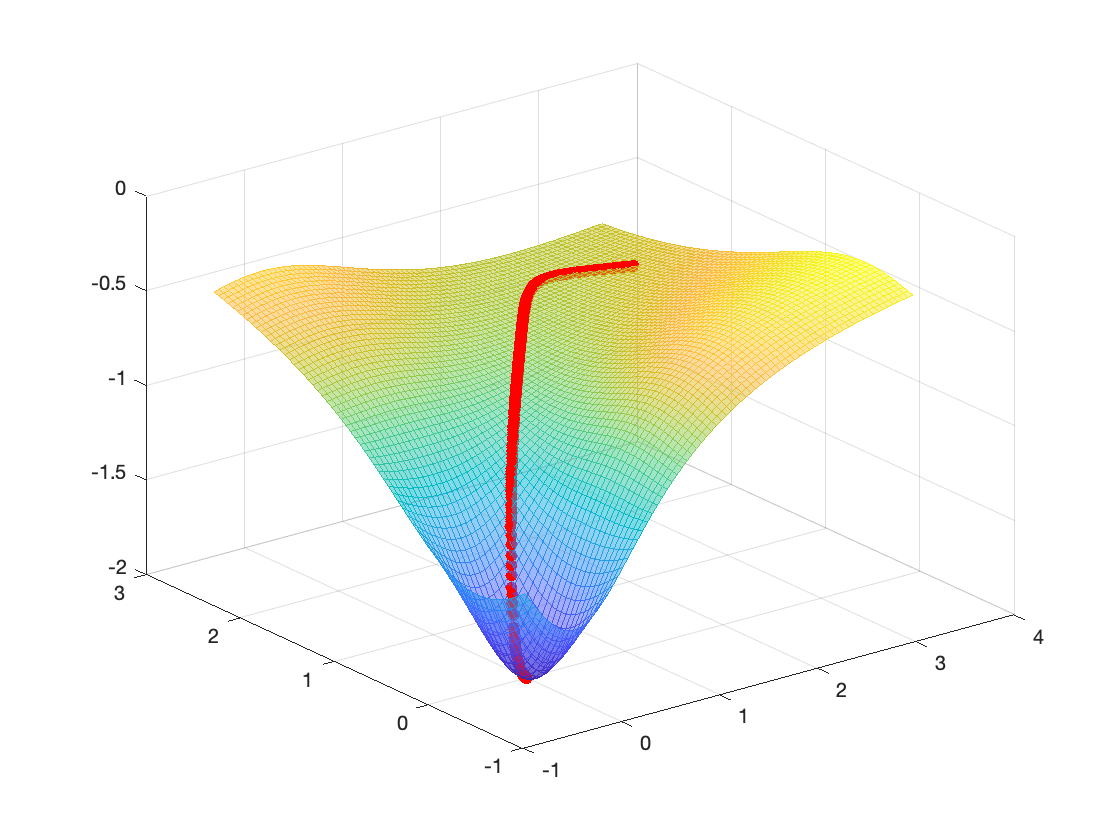
\includegraphics[width=0.4\linewidth]{figs/unc_2_sgd.png}\hfill
} 
\subfloat[Steepest Descent algorithm, using armijo stepsize rule selection(iteration = 8)]{
    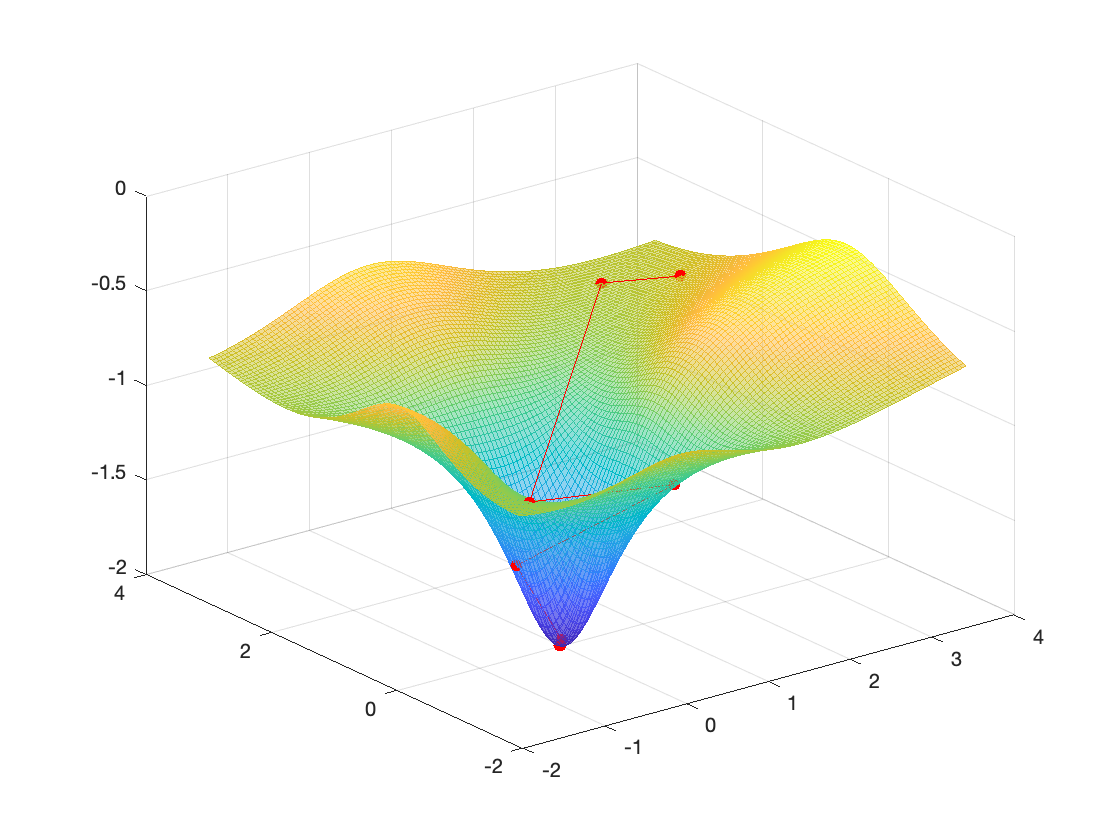
\includegraphics[width=0.4\linewidth]{figs/unc_2_sgd_armijo.png}\hfill
} \\
\subfloat[Conjugate Gradient algorithm\\(iteration = 23)]{
    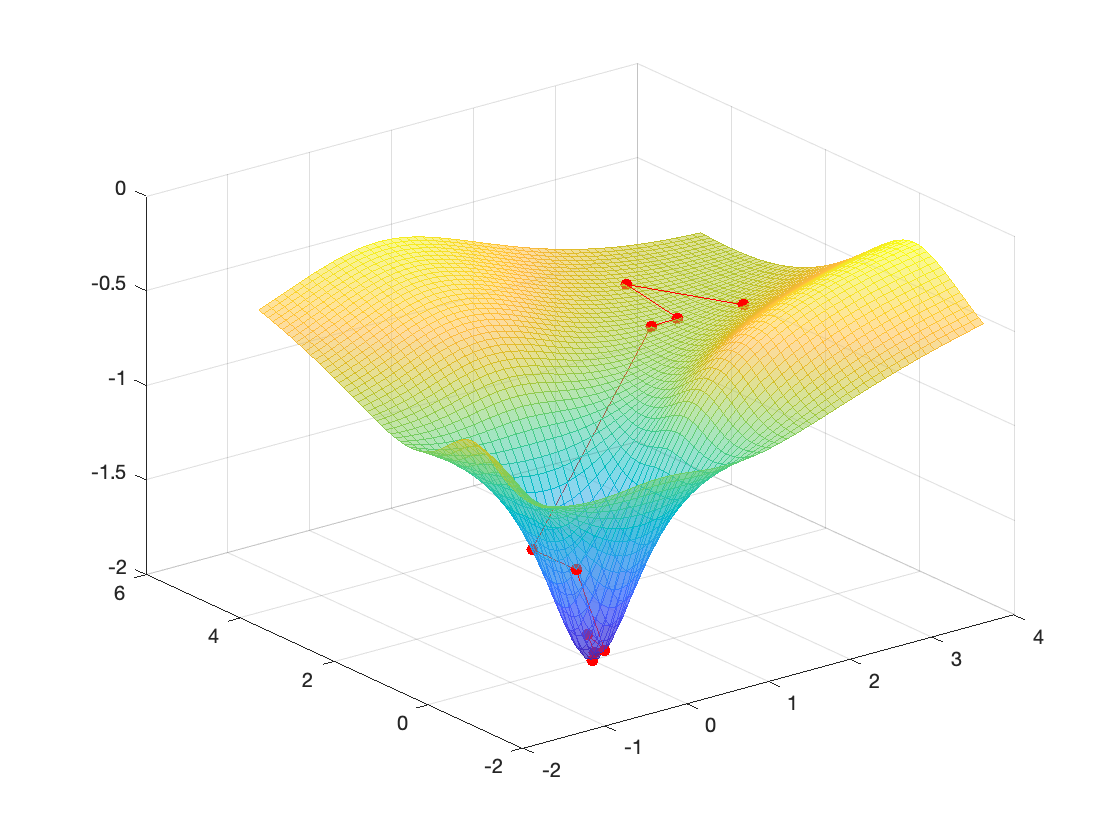
\includegraphics[width=0.4\linewidth]{figs/unc_2_cg.png}\hfill
} 
\subfloat[Secant algorithm\\(iteration = 9)]{
    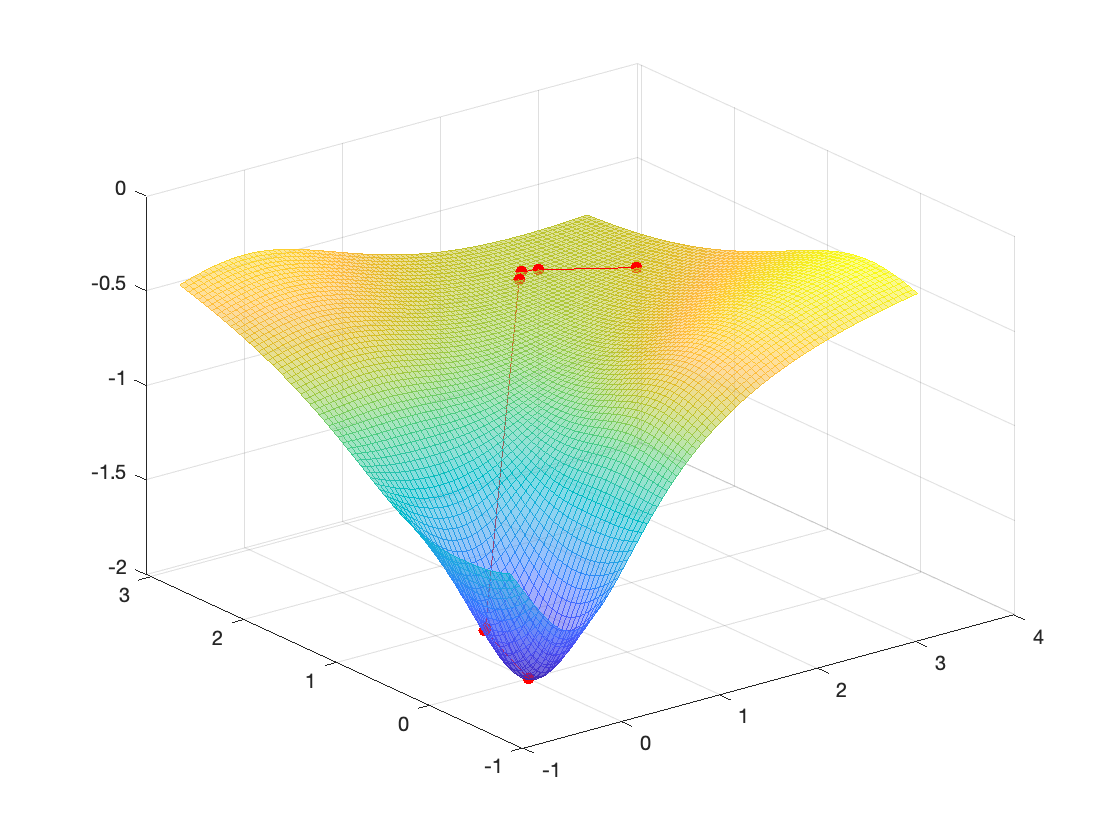
\includegraphics[width=0.4\linewidth]{figs/unc_2_secant.png}
}\hfill
\caption{unconstrained optimization problem(B) - initial point set to (3,2), and all graphs equally show convergence to minimizer(0,0) }
\label{unconstrained problem 2}
\end{figure}

Comparison between (a) and (b) on Figure\ref{unconstrained problem 2} in terms of number of total iteration to converge into a point indicates choosing proper step size can greatly reduce computational time by efficiently moving around the surface. 

\subsection*{problem(C) from EXAMPLE PROBLEMS}
Objective function to minimize :
\begin{equation}
  \begin{array}{l}
    V\left(x,y\right)=1+\left\lbrack \begin{array}{cc}
    1 & 2
    \end{array}\right\rbrack \left\lbrack \begin{array}{c}
    x\\
    y
    \end{array}\right\rbrack +\frac{1}{2}{\left\lbrack \begin{array}{c}
    x\\
    y
    \end{array}\right\rbrack }^T \left\lbrack \begin{array}{cc}
    12 & 3\\
    3 & 10
    \end{array}\right\rbrack \left\lbrack \begin{array}{c}
    x\\
    y
    \end{array}\right\rbrack \\
    +10\;\mathrm{ln}\left(1+x^4 \right)\mathrm{sin}\left(100x\right)+10\;\mathrm{ln}\left(1+y^4 \right)\mathrm{cos}\left(100x\right)\;;x,y\in R
  \end{array}
\end{equation}

The given function is a multivariable function with 2 input x and y. Algorithms are made to find minimum and its corresponding minimizer of 2d function.

\begin{figure}[ht!]%
\centering
\subfloat[Secant algorithm\\(iteration = 5)]{
    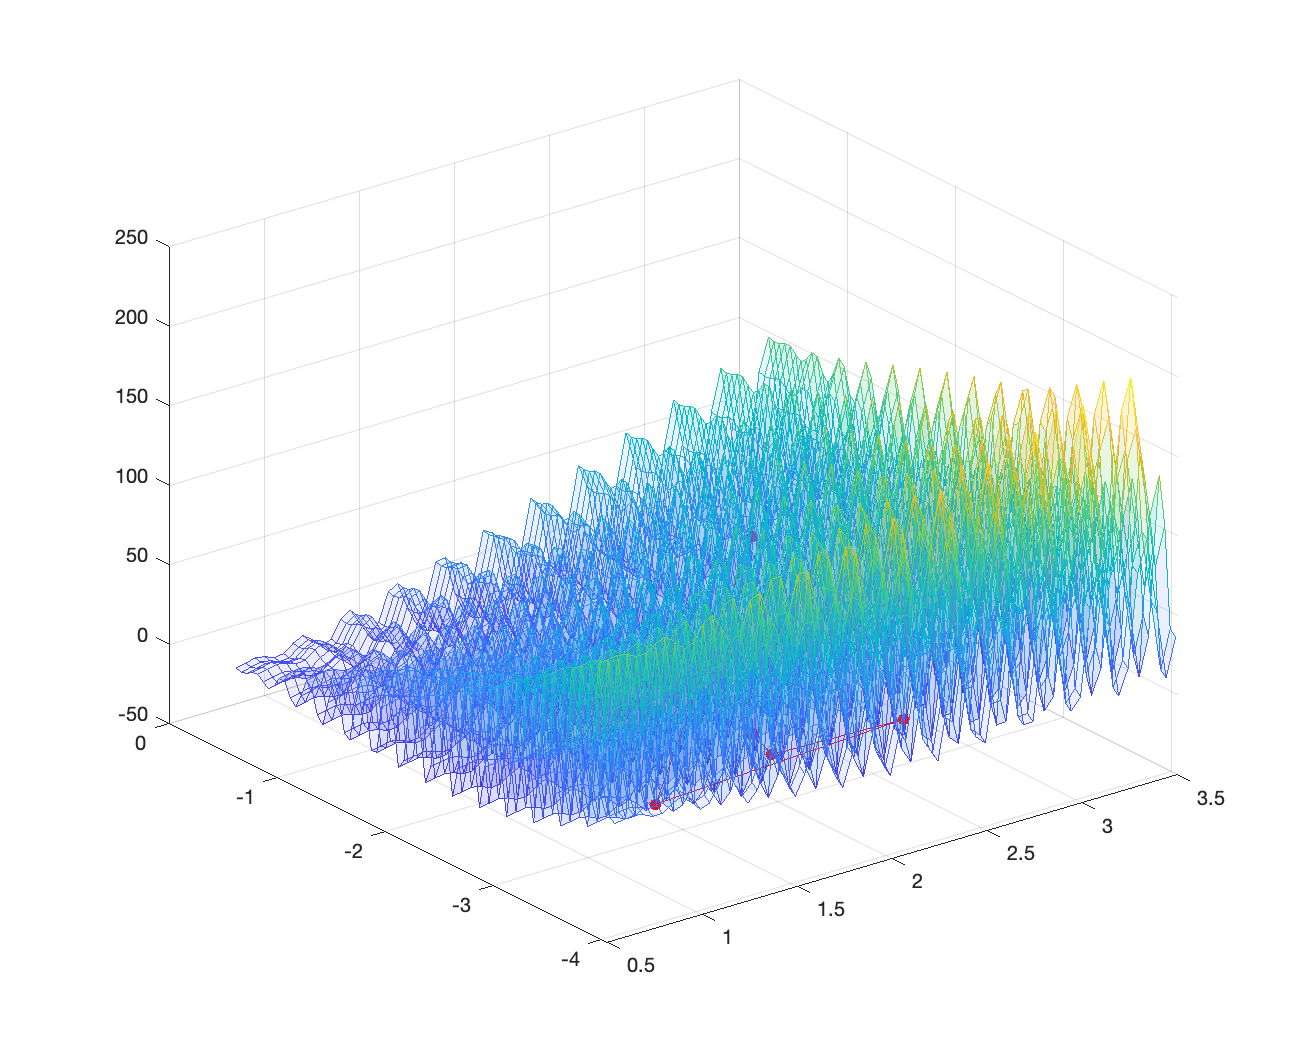
\includegraphics[width=0.48\linewidth]{figs/unc_3_secant.png}\hfill
} 
\subfloat[]{
    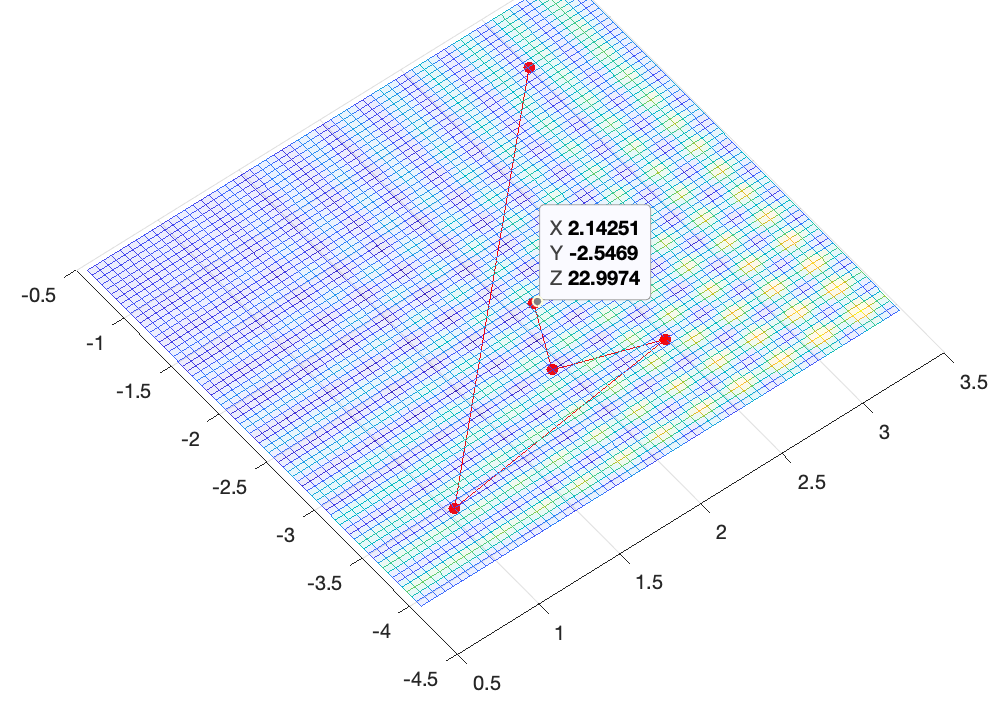
\includegraphics[width=0.48\linewidth]{figs/unc_3_secant2.png}\hfill
}
\caption{unconstrained optimization problem(C) - convergence to minimum }
\label{unconstrained problem 3}
\end{figure}

However, finding global minimum for this problem was extremely hard for all 4 algorithm, since the function has infinitely many local minimum with high frequency. Figure \ref{unconstrained problem 3} is a graph that shows path along iteration. It shows some kind of zig-zag pattern and have hard time finding local minimum.
\newpage

\section{Solving Constrained Optimization Problems}
\subsection*{problem(1) from PART 2}
Objective Function to minimize :
\begin{equation}
    \begin{array}{l}
    f_0(x,y)=|x-1|+|y-2|  ; x,y \in \mathbb{R} \\
    \end{array}
\end{equation}
Subject to :
\begin{equation}
    \begin{array}{l}
    h_1(x,y)=x-y^2 \ge 0 \\
    h_2(x,y)=x^2 +y^2 -1=0
    \end{array}
\end{equation}

The given function is a multivariable function with 2 input x and y, with one equality and one inequality constraint. Penalty function method can be used to solve this constrained optimization problem.
In penalty function, constant \texttt{alpha} that is multiplied to panelty function term increases from 10 to 10000 every iteration(10,20,50,100,200,500,1000,5000,10000, to be specific). There are total 9 iterations and every iteration, the algorithm searches global minimizer for temporary objective function(panelty function added to original objective function). To reduce computational time, MATLAB Optimization toolbox was used inside the loop.


\begin{figure}[!h]
    \centering
    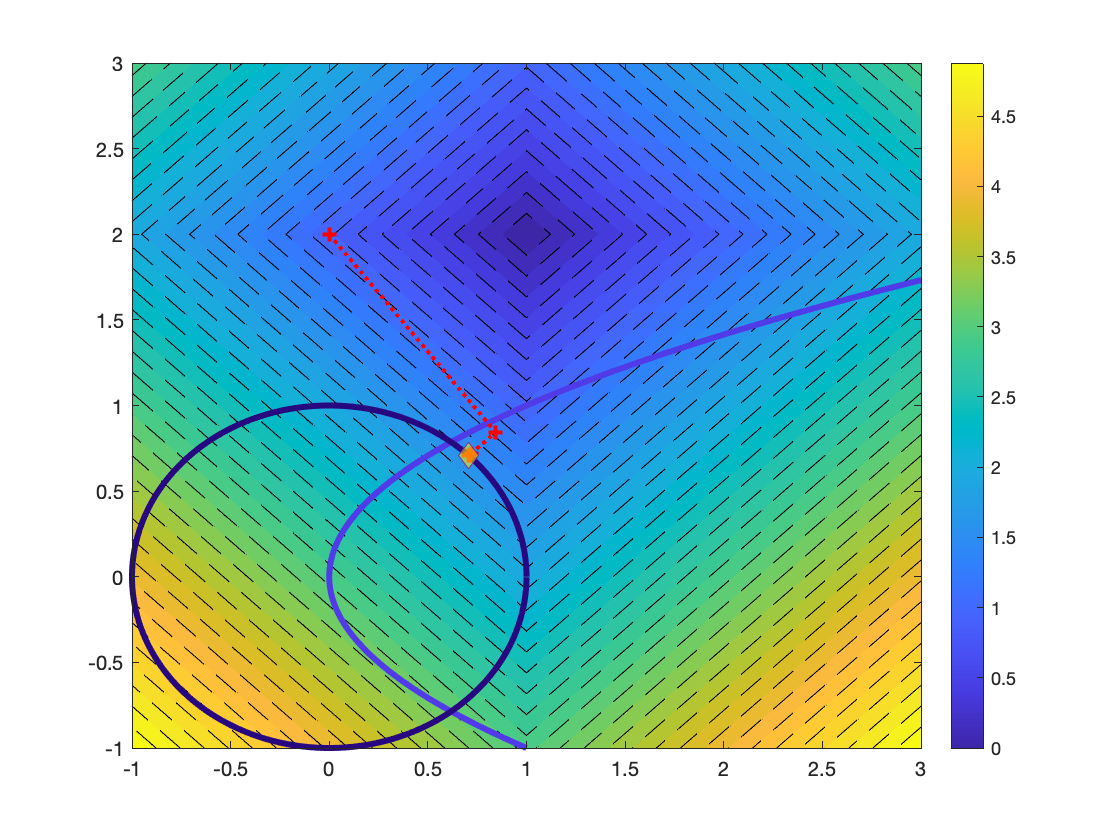
\includegraphics[width=0.7\textwidth]{figs/cst_1.png}
    \caption{Two dark blue line curves indicates boundary of two constraint $h_1(x,y)$ and $h_2(x,y)$. The red dots are global minimizer that are found each iteration, and yellow marked on (0.707,0.707) is the final estimated minimzer of the algorithm.}
\label{constrained problem 1}
\end{figure}

By randomly setting a initial point to start with, the penalty function method quickly finds the minimizer that are located in the constrained region. The initial point were set to (0,2), and the graph shows its convergence to minimizer(0.70712,0.70712). By observing contour lines(marked with dotted lines) of objective function and two constraints plotted on the 2D graph on Figure \ref{constrained problem 1}, we can intuitively confirm that the algorithm is properly finding minimum of the function that satisfies the constraints.

\subsection*{problem(2) from PART 2}
Objective Function to minimize :
\begin{equation}
    \begin{array}{l}
    f_0(x,y)=-xy  ; x,y \in \mathbb{R} \\
    \end{array}
\end{equation}
Subject to :
\begin{equation}
    \begin{array}{l}
    h_1(x,y)=x-y^2+1 \ge 0 \\
    h_2(x,y)=x+y \ge 0
    \end{array}
\label{cst2-h}
\end{equation}

The given function is a multivariable function with 2 input x and y, with two inequality constraints. Either Penalty or Barrier function method can be used to solve this constrained optimization problem. 
First, let's apply penalty function method to find minimum. The initial point is randomly selected to (2,-1) and Figure\ref{constrained problem 2} shows that the algorithm is correctly locating the minimum that satisfies every constraint.

\begin{figure}[!h]
    \centering
    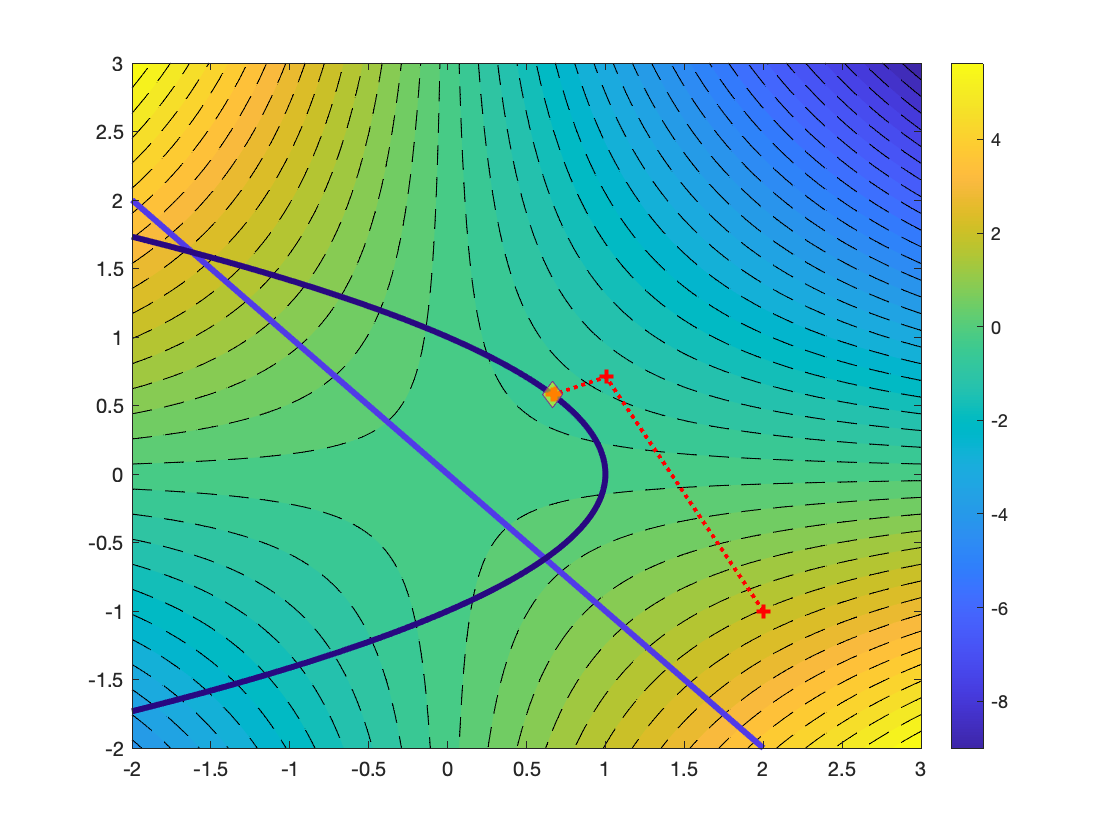
\includegraphics[width=0.7\textwidth]{figs/cst_2.png}
    \caption{Two dark blue line curves indicates boundary of two constraint $h_1(x,y)$ and $h_2(x,y)$. The red dots are global minimizer that are found each iteration, and yellow marked on(0.67,0.58) is the final estimated minimizer of the algorithm.}
\label{constrained problem 2}
\end{figure}

Next, we can try barrier function method since both constraints are in form of inequality. Initial point should be more carefully chosen than it did in penalty function since initial point should be located in feasible set to use barrier function method. A point (-0.5,1) satisfies every constraints in equation(\ref{cst2-h}), so let this point to be a starting point of iteration.\\
In barrier function, constant \texttt{beta} that is multiplied to panelty function term decreases from 100 to $10^{-5}$ every iteration(100,10,5,1,0.1,1e-2,1e-3,1e-4,1e-5, to be specific). There are total 9 iterations, and every iteration, the algorithm searches global minimizer for temporary objective function(barrier function added to original objective function) not considering any constraints. To reduce computational time, MATLAB Optimization toolbox was used inside the loop.

\begin{figure}[ht!]%
\centering
\subfloat[Penalty function method]{
    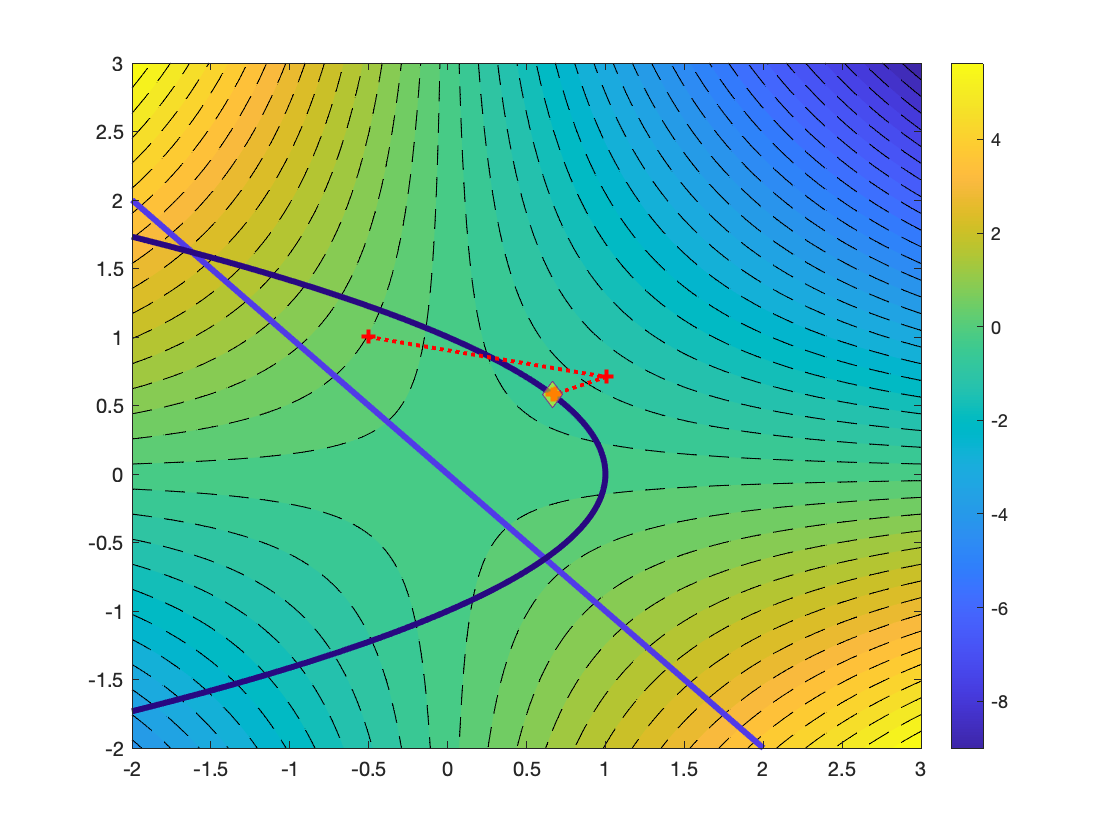
\includegraphics[width=0.48\linewidth]{figs/cst_2_penalty.png}\hfill
} 
\subfloat[Barrier function method]{
    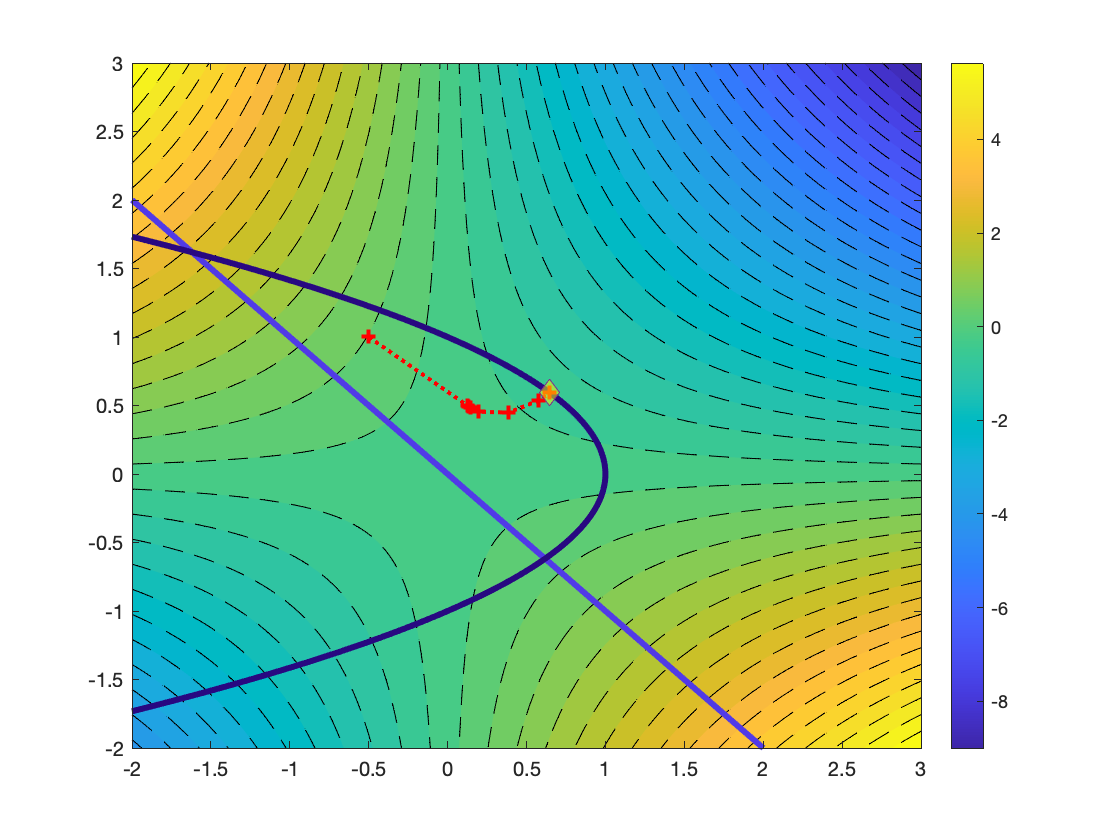
\includegraphics[width=0.48\linewidth]{figs/cst_2_barrier.png}\hfill
} 
\caption{constrained optimization problem(2) - Final minimizer estimation marked yellow is (0.67,0.58), (0.65,0.59) for penalty method and barrier method respectively. The path of estimated minimizer for every iteration differs from penalty function to barrier function method}
\label{constrained problem 2-barrier}
\end{figure}

Although both algorithm gives very similar estimation ultimately, the graphs above shows difference in their path. The largest difference between penalty and barrier function method is that in barrier method, estimated minimizer(marked in red) stays inside the boundary of constraints and slowly move towards the barrier with smaller value, whereas in penalty method, estimated minimizer tends to starts from the minimizing point without any constraints and then move towards the constraints boundary.

By observing contour lines(marked with dotted lines) of objective function and two constraints plotted on the 2D graph on Figure \ref{constrained problem 1}, we can intuitively confirm that the algorithm is properly finding minimum of the function that satisfies the constraints.

\subsection*{problem(3) from PART 2}
Objective Function to minimize :
\begin{equation}
    \begin{array}{l}
    f_0(x,y)= ln(x)-y  ; x,y \in \mathbb{R} \\
    \end{array}
\end{equation}
Subject to :
\begin{equation}
    \begin{array}{l}
    h_1(x,y)=x-1 \ge 0 \\
    h_2(x,y)=x^2 +y^2 -4=0
    \end{array}
\end{equation}

The given function is a multivariable function with 2 input x and y, with one equality and one inequality constraint. Penalty function method can be used to solve this constrained optimization problem.


\begin{figure}[!h]
    \centering
    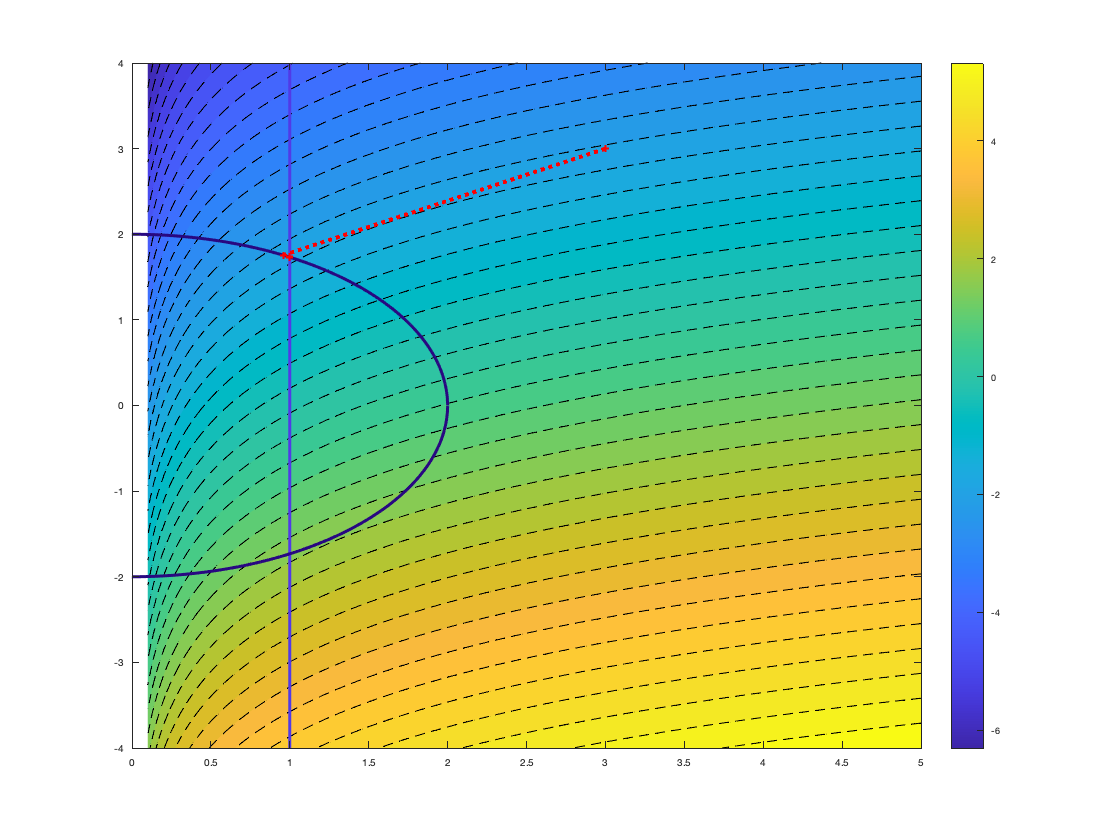
\includegraphics[width=0.7\textwidth]{figs/cst_3.png}
    \caption{Two dark blue line curves indicates boundary of two constraint $h_1(x,y)$ and $h_2(x,y)$. The red dots are global minimizer that are found each iteration, and yellow marked on (1,1.732) is the final estimated minimzer of the algorithm.}
\label{constrained problem 1}
\end{figure}

 By observing contour lines(marked with dotted lines) of objective function and two constraints plotted on the 2D graph on Figure \ref{constrained problem 1}, we can intuitively confirm that the algorithm is properly finding minimum of the function that satisfies the constraints.

Since the given objective function has neither global nor local minimum if there's no constraints, alpha value should be carefully chosen to assure convergence of the algorithm.

\end{document}